% Options for packages loaded elsewhere
\PassOptionsToPackage{unicode}{hyperref}
\PassOptionsToPackage{hyphens}{url}
\PassOptionsToPackage{dvipsnames,svgnames,x11names}{xcolor}
%
\documentclass[
  12pt]{article}

\usepackage{amsmath,amssymb}
\usepackage{lmodern}
\usepackage{iftex}
\ifPDFTeX
  \usepackage[T1]{fontenc}
  \usepackage[utf8]{inputenc}
  \usepackage{textcomp} % provide euro and other symbols
\else % if luatex or xetex
  \usepackage{unicode-math}
  \defaultfontfeatures{Scale=MatchLowercase}
  \defaultfontfeatures[\rmfamily]{Ligatures=TeX,Scale=1}
\fi
% Use upquote if available, for straight quotes in verbatim environments
\IfFileExists{upquote.sty}{\usepackage{upquote}}{}
\IfFileExists{microtype.sty}{% use microtype if available
  \usepackage[]{microtype}
  \UseMicrotypeSet[protrusion]{basicmath} % disable protrusion for tt fonts
}{}
\makeatletter
\@ifundefined{KOMAClassName}{% if non-KOMA class
  \IfFileExists{parskip.sty}{%
    \usepackage{parskip}
  }{% else
    \setlength{\parindent}{0pt}
    \setlength{\parskip}{6pt plus 2pt minus 1pt}}
}{% if KOMA class
  \KOMAoptions{parskip=half}}
\makeatother
\usepackage{xcolor}
\setlength{\emergencystretch}{3em} % prevent overfull lines
\setcounter{secnumdepth}{5}
% Make \paragraph and \subparagraph free-standing
\ifx\paragraph\undefined\else
  \let\oldparagraph\paragraph
  \renewcommand{\paragraph}[1]{\oldparagraph{#1}\mbox{}}
\fi
\ifx\subparagraph\undefined\else
  \let\oldsubparagraph\subparagraph
  \renewcommand{\subparagraph}[1]{\oldsubparagraph{#1}\mbox{}}
\fi


\providecommand{\tightlist}{%
  \setlength{\itemsep}{0pt}\setlength{\parskip}{0pt}}\usepackage{longtable,booktabs,array}
\usepackage{calc} % for calculating minipage widths
% Correct order of tables after \paragraph or \subparagraph
\usepackage{etoolbox}
\makeatletter
\patchcmd\longtable{\par}{\if@noskipsec\mbox{}\fi\par}{}{}
\makeatother
% Allow footnotes in longtable head/foot
\IfFileExists{footnotehyper.sty}{\usepackage{footnotehyper}}{\usepackage{footnote}}
\makesavenoteenv{longtable}
\usepackage{graphicx}
\makeatletter
\def\maxwidth{\ifdim\Gin@nat@width>\linewidth\linewidth\else\Gin@nat@width\fi}
\def\maxheight{\ifdim\Gin@nat@height>\textheight\textheight\else\Gin@nat@height\fi}
\makeatother
% Scale images if necessary, so that they will not overflow the page
% margins by default, and it is still possible to overwrite the defaults
% using explicit options in \includegraphics[width, height, ...]{}
\setkeys{Gin}{width=\maxwidth,height=\maxheight,keepaspectratio}
% Set default figure placement to htbp
\makeatletter
\def\fps@figure{htbp}
\makeatother

\addtolength{\oddsidemargin}{-.5in}%
\addtolength{\evensidemargin}{-1in}%
\addtolength{\textwidth}{1in}%
\addtolength{\textheight}{1.7in}%
\addtolength{\topmargin}{-1in}%
\makeatletter
\makeatother
\makeatletter
\makeatother
\makeatletter
\@ifpackageloaded{caption}{}{\usepackage{caption}}
\AtBeginDocument{%
\ifdefined\contentsname
  \renewcommand*\contentsname{Table of contents}
\else
  \newcommand\contentsname{Table of contents}
\fi
\ifdefined\listfigurename
  \renewcommand*\listfigurename{List of Figures}
\else
  \newcommand\listfigurename{List of Figures}
\fi
\ifdefined\listtablename
  \renewcommand*\listtablename{List of Tables}
\else
  \newcommand\listtablename{List of Tables}
\fi
\ifdefined\figurename
  \renewcommand*\figurename{Figure}
\else
  \newcommand\figurename{Figure}
\fi
\ifdefined\tablename
  \renewcommand*\tablename{Table}
\else
  \newcommand\tablename{Table}
\fi
}
\@ifpackageloaded{float}{}{\usepackage{float}}
\floatstyle{ruled}
\@ifundefined{c@chapter}{\newfloat{codelisting}{h}{lop}}{\newfloat{codelisting}{h}{lop}[chapter]}
\floatname{codelisting}{Listing}
\newcommand*\listoflistings{\listof{codelisting}{List of Listings}}
\makeatother
\makeatletter
\@ifpackageloaded{caption}{}{\usepackage{caption}}
\@ifpackageloaded{subcaption}{}{\usepackage{subcaption}}
\makeatother
\makeatletter
\@ifpackageloaded{tcolorbox}{}{\usepackage[many]{tcolorbox}}
\makeatother
\makeatletter
\@ifundefined{shadecolor}{\definecolor{shadecolor}{rgb}{.97, .97, .97}}
\makeatother
\makeatletter
\makeatother
\ifLuaTeX
  \usepackage{selnolig}  % disable illegal ligatures
\fi
\usepackage[]{natbib}
\bibliographystyle{agsm}
\IfFileExists{bookmark.sty}{\usepackage{bookmark}}{\usepackage{hyperref}}
\IfFileExists{xurl.sty}{\usepackage{xurl}}{} % add URL line breaks if available
\urlstyle{same} % disable monospaced font for URLs
\hypersetup{
  pdftitle={Introductory Data Science: A Blueprint to Design Curriculum and Pedagogy},
  pdfauthor={Elijah Meyer; Mine Çetinkaya-Rundel},
  pdfkeywords={Data Science, Curriculum, Pedagogy},
  colorlinks=true,
  linkcolor={blue},
  filecolor={Maroon},
  citecolor={Blue},
  urlcolor={Blue},
  pdfcreator={LaTeX via pandoc}}


\begin{document}


\def\spacingset#1{\renewcommand{\baselinestretch}%
{#1}\small\normalsize} \spacingset{1}


%%%%%%%%%%%%%%%%%%%%%%%%%%%%%%%%%%%%%%%%%%%%%%%%%%%%%%%%%%%%%%%%%%%%%%%%%%%%%%

\date{July 7, 2023}
\title{\bf Introductory Data Science: A Blueprint to Design Curriculum
and Pedagogy}
\author{
Elijah Meyer\\
Department of Statistics, Duke University\\
and\\Mine Çetinkaya-Rundel\\
Department of Statistics, Duke University\\
}
\maketitle

\bigskip
\bigskip
\begin{abstract}
The text of your abstract. 200 or fewer words.
\end{abstract}

\noindent%
{\it Keywords:} Data Science, Curriculum, Pedagogy
\vfill

\newpage
\spacingset{1.9} % DON'T change the spacing!
\ifdefined\Shaded\renewenvironment{Shaded}{\begin{tcolorbox}[interior hidden, boxrule=0pt, borderline west={3pt}{0pt}{shadecolor}, sharp corners, breakable, enhanced, frame hidden]}{\end{tcolorbox}}\fi

\hypertarget{introduction}{%
\section{Introduction}\label{introduction}}

\textbf{TO DO: Implement blinding}

The demand for data science is here. An estimated 11.5 million new data
science jobs are projected to be created by 2026, while employment of
data scientists is projected to grow by 36 percent from 2021 to 2031
\citep{labor_2022}. As job market demands increase, so do the demands in
academia. This is a call for universities to offer such courses to best
prepare students in data science, and to be prepared for class sizes to
increase. The increasing volume of enrollment of data science students
\citep{Redmond2022} requires that statistics and data science educators
commit to developing modern curriculum in order to help students be
successful. Despite the demand, academics are still struggling with what
a modern data science curriculum should look like \citep{Schwab2020},
and how it can be effectively taught to a large student audience. To
this point, much more thought, work, and discussions need to take place
before a consensus is reached on what a modern data science curricula
should look like.

To answer this call, the Curriculum Guidelines for Undergraduate
Programs in Data Science provided six major recommendations as to what
practitioners of data science should be competent in: computational and
statistical thinking, mathematical foundations, model building and
assessment, algorithms and software foundation, data curation,
communication and responsibility \citep{veaux_2017}. Additionally, the
Association for Computing Machinery Education Council's Data Science
Task Force explores and expands discipline-specific conversations around
the field of data science \citep{Danyluk_2021}. This task force
acknowledges that data science curricula can be flexible, but suggests
that data science curricula should include applications designed towards
building skills in computing, statistics, machine learning and
mathematics.

However, it is difficult to create a new course. It becomes even more
challenging to create a course in-tune to the guidelines above. Thus,
many of the recommendations are not being observed, with the majority of
current curricula largely focusing on how to model data
\citep{Donoho2017}. The picture becomes even less clear on what context
constitutes a well developed modernized introductory data science
course. As the demand for data science trickles down from the work force
into university, it is critical that students' initial experiences with
introductory data science helps inspire students into this field, and
ensure they are best prepared for future courses.

This presents a need for a \emph{blueprint} to design and implement and
modernized introduction to data science course that lays the foundation
for students to develop an encompassing data science skill set. In this
paper, we lay out this blueprint, while addressing realistic challenges
both we have faced and other instructors may face when developing,
creating, and implementing an introductory data science course. This
discussion is through the lens of a modernized data science curricula
for an introductory data science course at Duke University.

This course is designed for large class sizes that enrolls students with
little to no statistics, data science, or coding experience, common
hurdles identified by faculty when trying to implement a data science
course \citep{Schwab2020}. By the end of this course, students are
expected and able to clean, investigate, and communicate with data in a
reproducible manner. Detailed learning objectives of this course include
learning to explore, visualize, and analyze data in a reproducible and
shareable manner through the use of RStudio and GitHub
\citep{R21, github}. Through these programs, students gain experience in
data wrangling, exploratory data analysis, predictive modeling, and data
visualization.

In this paper, we discuss the creation and implementation of curricular
and pedagogical decisions made in designing the introductory data
science course at Duke University. This includes detailing the
implementation of our student learning model to support a large class of
students with a diverse background in statistics, data science, and
coding experience. Additionally, we provide examples of and describe
activities and assessments given both in and outside of class. We extend
discussions and provide recommendations for implementing and integrating
computing tools, such as RStudio and GitHub, through our experiences in
our course. Lastly, we discuss challenges, and provide insight to help
instructors wanting to adopt or adapt a course similar to introductory
to the one we describe. The purpose of this paper is to create a
discussion around a modernized curricula for an introductory data
science course, and the pedagogical decisions to help best excite and
equip students with the data science skills necessary for future
classes. We aim to help instructors adopt, adapt, and make decisions
towards their own introductory data science course to best fit their
university.

\hypertarget{sec-course}{%
\section{The Course}\label{sec-course}}

The design of this course is largely influenced by the \textbf{data
science in a box} design principles (cite). This includes inspiring
students early by showing students the ``end result'', and encourage
students to make their first meaningful data visualization on day one.
In the following sections, we provide a flexible ``first-person''
perspective blueprint for course creation, modernization, and
implementation through the lens of our introductory data science course
at Duke University. For more general information on the leading design
principles of this course, please see the data science in a box design
principles
\href{https://datasciencebox.org/01-design-principles.html}{here}.

Our course, titled \textbf{Introduction to Data Science and Statistical
thinking} (STA199), often houses students undecided on their major, but
have interests that span across topics such as public policy, biology,
computer science, nursing, and statistics. Commonly, most students have
little to no statistics, data science, or coding experience. In a
typical semester, this course seats roughly 150 students, which is
considered to be large by all measures. Both the lack of experience and
large class size are identified as two common hurdles by faculty when
trying to create and instruct an introductory data science course
\citep{Schwab2020, Kok_2008}. However, by the end of this course,
students are able to use both the statistical software R and GitHub to
create data visualizations, investigate patterns, and model outcomes in
a reproducible format.

This course is built on four large-scale learning objectives: learn to
explore, visualize and analyze data in a reproducible and shareable
manner; gain experience in data wrangling and munging, exploratory data
analysis, predictive modeling, and data visualization; work on problems
and case studies inspired by and based on real-world questions and data;
learn to effectively communicate results through written assignments and
project presentation. These objectives are accomplished through
interactive lectures and labs that present content, problems, and case
studies inspired by and based on real-world questions and data.

When teaching, instructors are committed to helping students build up a
foundation of knowledge that sets the stage for each student to not only
accomplish tasks, but train their brain to work through complex
statistical and coding problems (Figure 1).

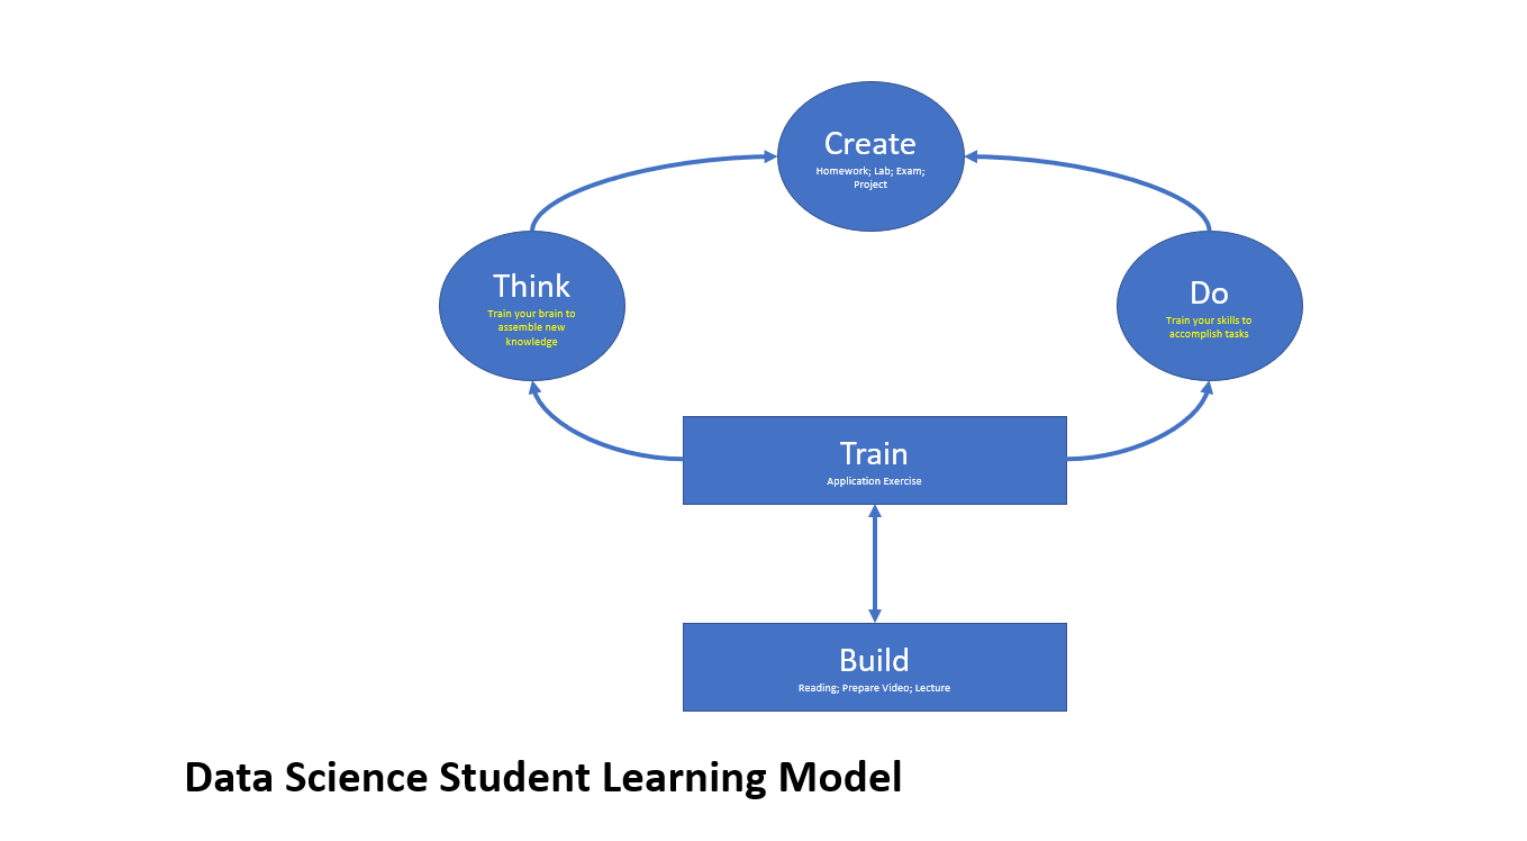
\includegraphics{images/learning_model.png} \textbf{Fig 1:} Data Science
Student Learning Model for STA 199

This model yields five components that are woven into the student
learning structure of this course. In the initial phase, students are
first introduced to content through assigned readings, videos, and
lectures. During this, students learn through multiple modes of
teaching, and create a foundation of information that they can continue
to build upon. They build upon existing knowledge by \emph{training}
their brain through interactive hands on in-class application exercises.
During these exercises, students are given in-class opportunities to
solve problems individually, as a group, and at the class level. During
this time, there is emphasis placed both on the \emph{doing}, or steps
needed to accomplish the task, as well as the \emph{thinking}, or
training of the brain to accomplish similar tasks in the future. This
culminates into assessments that allow students to show the what they
have learned, and connections they can make with the material.
Assessments include homeworks, quizzes, exams, and project components.

This model is designed to both situate the student and guide the
instructor in facilitating an overall quality learning experience. This
learning model outlines a process performed during a typical week within
a semester.

Topics taught through this cycle fall under for major units: Exploring
data; Data science ethics; Making rigorous conclusions; Looking further
\textbf{(cite dsbox?)}. In the first two units, students are introduced
to R, RStudio, and Github. During exploring data, students start to
create data visualizations and learn how to both import and manipulate
data to be better suited for modeling. Next, multiple classes are spent
having conversations around and facilitating activities on the topic of
data ethics to help ensure students start developing the skills
necessary to be responsible researchers. In the next two units, students
extend their investigations and understandings of data into a modeling
framework. Specifically, students fit a variety of models (simple linear
regression, multiple linear regression, logistic regression), and learn
the fundamentals of hypothesis testing and confidence intervals. The
looking further section includes independent topics that the instructor
can choose to teach, typically at the end of the semester. Topics have
included cryptanalysis and genetic forensic analysis, visualizing
spatial data, Bayesian inference, creating interactive web applications
with Shiny, and text analysis and text modeling. The goal of these
lessons are to provide an opportunity to have students learn about
topics that interest them in a no-stakes environment, continuing to
excite and inspire students into a career in statistics and data
science. For more information specific to the course content, please
refer to the following paper
\href{https://www.tandfonline.com/doi/epdf/10.1080/10691898.2020.1804497?needAccess=true\&role=button}{here}
\citep{Cetinkaya2020}.

\hypertarget{implementation}{%
\section{Implementation}\label{implementation}}

In the following sections, we describe the preparation and
implementation process necessary to run STA 199, in its entirety. This
includes details of a teaching team used to instruct, technology we've
chosen to use, as well as our pedagogical choices that go into a typical
week of teaching. This comprehensive description is encouraged to be
used as a flexible framework on how to create, set up, and implement an
introduction to data science course similar to STA 199. In this
description, we articulate first hand experiences, suggestions, and
provide example code and lessons that aim to support newer instructors
who are developing or teaching an introductory data science course;
instructors with courses that are increasing in size; and instructors
who want to implement more technical tools into their curricula and
classroom.

\hypertarget{teaching-team}{%
\subsection{Teaching Team}\label{teaching-team}}

We structure a teaching team to help account for the difficulties a
large class size can bring. Our teaching team consists of one instructor
and multiple teaching assistants (TAs). The responsibilities of any TA
is to both support the instructor in charge of the class, and support
the students in the classroom. These TAs range from undergraduate to
PH.D. level students, and vary in teaching experience. \textbf{(Writing
on TA selection process). Once selected\ldots{} (writing on TA
training).}

Once training is complete, TAs are assigned roles that indicate their
responsibilities during the semester. These roles include \emph{course
organizer}, \emph{head TA}, \emph{lab leader}, and \emph{lab helper}.
Often, these roles are given based on the academic level of student,
with more academically experienced TAs taking on the roles of course
organizer, head TA, and lab leader, where as students with less
experience (i.e.~undergraduate students) take on the role of lab helper.

Lab sections are held once a week, and are facilitated in person by both
a lab leader and lab helper. The responsibilities of a lab helper are
supporting both the students and lab leader as they see fit. Examples of
this may include setting up the classroom before class, or conducting
small group conversations when students have questions about the
material. The lab leader is responsible for facilitating the lab. This
may involve giving a brief introduction and wrap up of lab content, as
well as being able to answer questions and facilitate conversations
among students about the lab assessment material. In addition, both must
hold two hours of office hours each week and have grading
responsibilities assigned throughout the semester.

Head TA responsibilities can generally be categorized into the following
categories: Administrative and pedagogical. Administrative
responsibilities include the organization and distribution of TA
responsibilities throughout the semester. It is imperative that the head
TA and instructor clearly communicate expectations with each other to
establish exactly how rules and responsibilities are assigned to TAs.
This includes distributing grading assignments and deadlines to both lab
helpers and leaders, weekly. The head TA also makes sure that all TAs
complete grading within a week and spot check the grading accuracy and
quality of all written feedback given. Other administrative duties
include reminding other TAs about bi-weekly payroll deadlines and ensure
TAs are working their alloted hours per week (and not more).
Pedagogically, head TAs are responsible for creating or reviewing answer
keys and grading rubrics for homework and lab assessments as the
instructor sees fit. Each head TA is also assigned to instruct one lab
section during the semester. Before becoming a Head TA, there is
additional training that specializes head TAs in their administrative
responsibilities.

The course organizer is expected to work across each section of STA 199,
instead of working with a single instructor. Their responsibilities
include creating rubrics for and working through homework and lab
assignments. Additionally the course organizer, along with the
instructor, answers real time questions virtually during labs asked by
lab leaders. Questions often range from content related to technical
questions about GitHub and R. Finally, the course organizer is
responsible for handling all requested assignment extensions from
students. This includes filing away student exemptions, providing
extensions for extreme circumstances, and enforcing the late work policy
outlined in the syllabus when necessary.

We typically have one course organizer, one head TA, six lab leaders,
and six lab helpers. Although this is our proposed team structure, we
want to emphasize that there is great flexibility in coming up with how
a teaching team is built and operates for an introductory to data
science course. Among any team, we encourage a system designed to
alleviate the grading responsibilities of a large class from a single
individual, dispersed into many among the team. When grading, it is
suggested that each individual is properly trained on how to grade
assessments, and expectations on how to provide feedback are clear.
Unclear feedback given has often been a point of contention from
students in the past. For each assignment, we recommend having one
member of the team grade one problem across the entirety of the class
roster. This helps adhere to more consistent grading, and encourages
more grading questions to be asked as they arise, earlier in the grading
process.

Through our experiences, it has been imperative that everyone within the
team is communicating with each other. A team with many different roles
poses risk for the instructor to be unaware of how or what decisions are
being enacted at the grading and lab levels of the course. Thus, it is
recommended that the instructor trains everyone on the teaching team to
use a communication system that allows every member to communicate any
questions they may have, or decisions they make, to the entire team. In
the past, we have used the software \emph{Slack}, with appropriately
named channels such as \emph{grading-questions}, where TAs can post
grading examples and questions about grading so the instructor can
clearly respond with their expectations. Further, it should be noted
that the head TA should not be treated as a ``bridge of communication''
for the instructor to the rest of the teaching team. It is critical that
that the instructor is in consistent contact with all members of the
teaching team in making sure all lab leaders and helpers understand the
course content, how to grade, and know what's expected of them in their
assigned role. We recommend holding a weekly meeting with all members of
the teaching team to ensure this. When members are unable to come, it is
an expectation that they watch a recorded video of the meeting and reach
out if they have any questions about what was discussed.

\hypertarget{sec-tech}{%
\subsection{Technology}\label{sec-tech}}

We use R, RStudio, and GitHub to create interactive lessons, and assign
pre-created assessments to individual or groups of students. In the
following sections, we detail the computing infrastructure needed to do
so. This includes details and examples with R, RStudio, and GitHub, from
the instructor's perspective, to set up lectures, AEs, labs and
homework. First, we justify our decision to use GitHub in STA 199 before
detailing necessary steps and student information needed so creation can
take place.

\hypertarget{why-github}{%
\subsubsection{Why GitHub}\label{why-github}}

We choose to use GitHub for STA 199 because it easily and efficiently
allows us to create and administer assessments and interactive lessons
to a large class size in individual GitHub repositories. Further, within
these repositories, instructors can provide template code and other
resources necessary to best facilitate an interactive lesson where
students can code together with the instructor during lecture.
Additionally, teaching through GitHub provides the ability to re-use
what you currently create as a template for subsequent semesters. Thus,
this system both rewards and encourages time investment into the
creation of assessments and lesson plans.

From the student perspective, exposing them to version control software
early in their academic career helps them develop good habits as
researchers and emphasize the importance of reproducibility in science.

\hypertarget{why-r-rstudio}{%
\subsection{Why R \& RStudio}\label{why-r-rstudio}}

R is a statistical programming language for computing and modeling while
RStudio is an integrated development environment for R \citep{Rcite}. We
choose these resources because they integrate seamlessly with GitHub,
and provide the instructor efficient tools to be used to distribute
assessments and in-class activities to students.

Further, there are many benefits to introduce these technology from the
student perspective. First, they are freely available to download and
are currently in high demand in different data science job
opportunities. In addition, this programming language has a
comprehensive library of packages that allows students to create data
visualizations and seamlessly analyze data, aligning with our learning
objectives for the course. Further, this software is compatible with
online versions that students can access without having to go through a
local installment if they do not wish or are unable. There exists online
versions that can be set up for students, with capabilities of
pre-populating their software with the appropriate packages needed for
the semester. Addressing these hurdles for students early is
advantageous any instructor who is working with a large amount of
students that are inexperienced with coding.

\hypertarget{setting-up-students-r-rstudio}{%
\subsubsection{Setting Up Students R \&
RStudio}\label{setting-up-students-r-rstudio}}

In an introductory course, it is recommended to minimize student
frustration and distraction through the use of pre-packaged
computational infrastructure \citep{Rundel2018}. Per this
recommendation, STA 199 has students use R and RStudio through a
\emph{Duke Container}. Duke containers provides instructors at Duke
university the opportunity to facilitate the use of different software,
such as R and RStudio, through an online container instead of needing
students to locally download both programs. Additionally, instructors
have the ability to manage and install packages students will need for
the semester, helping provide a neat and well organized starting
experience with a new statistical language. \textbf{(insert discussion
on how this is done)}.

\textbf{(Transition to RStudio cloud discussion? What alternatives can
instructors use to imitate Duke containers if this is something they do
not have access to at their university.)}

\hypertarget{setting-up-a-github-account}{%
\subsubsection{Setting up a GitHub
account}\label{setting-up-a-github-account}}

To participate in interactive lessons and assessments, students must set
up a GitHub account. This is done of the first day of class, and often,
students are given time during class to sign up. Following tips from
``Happy Git with R'' \citep{bryan_hester_2020}, we suggest students do
the following when creating their name:

-- Incorporate their actual name

-- Reuse their username from other contexts if you can

-- Pick a username they will be comfortable revealing to a future boss

-- Be as unique as possible in as few characters as possible. Shorter is
better than longer

-- Avoid words with special meaning in programming (i.e., NA)

Once students create their account, we suggest getting this information
from them in a survey. This normally can be done through your learning
management system. It is critical to reiterate to students that spelling
and capitalization matter when they provide their GitHub username. We
suggest asking the question as follows:

\textbf{(should we include the questions in a highlighted text box of
some sort?)}

\textbf{What is your GitHub username?}

\textbf{Answer this question by ONLY typing your GitHub name and nothing
else.}

\textbf{Make sure you triple-check the spelling so I don't add random
strangers to our course organization on GitHub}

Once this information is collected, it must be exported and stored as a
\texttt{.csv} file to be read into R later. We recommend having the
following structure of data collected from the survey.

\begin{longtable}[]{@{}lll@{}}
\toprule()
\endhead
last\_name & first\_name & github\_username \\
& & \\
\bottomrule()
\end{longtable}

\textbf{Fig 2: Example Data Collection}

If you, as the instructor, do not have a GitHub account, you will need
to create one as well. This student information will be used to enroll
students in your created GitHub organization for your course.

\hypertarget{github-organization}{%
\subsubsection{GitHub organization}\label{github-organization}}

GitHub organizations are shared accounts where instructors and students
can collaborate across many projects at once. When designing your
course, we suggest running it through a GitHub organization that is
managed with R \& R-studio. This way, students will gain experience with
a modern statistical toolkit, and you, as the instructor, can
efficiently distribute assessments to individual students (Figure 2).

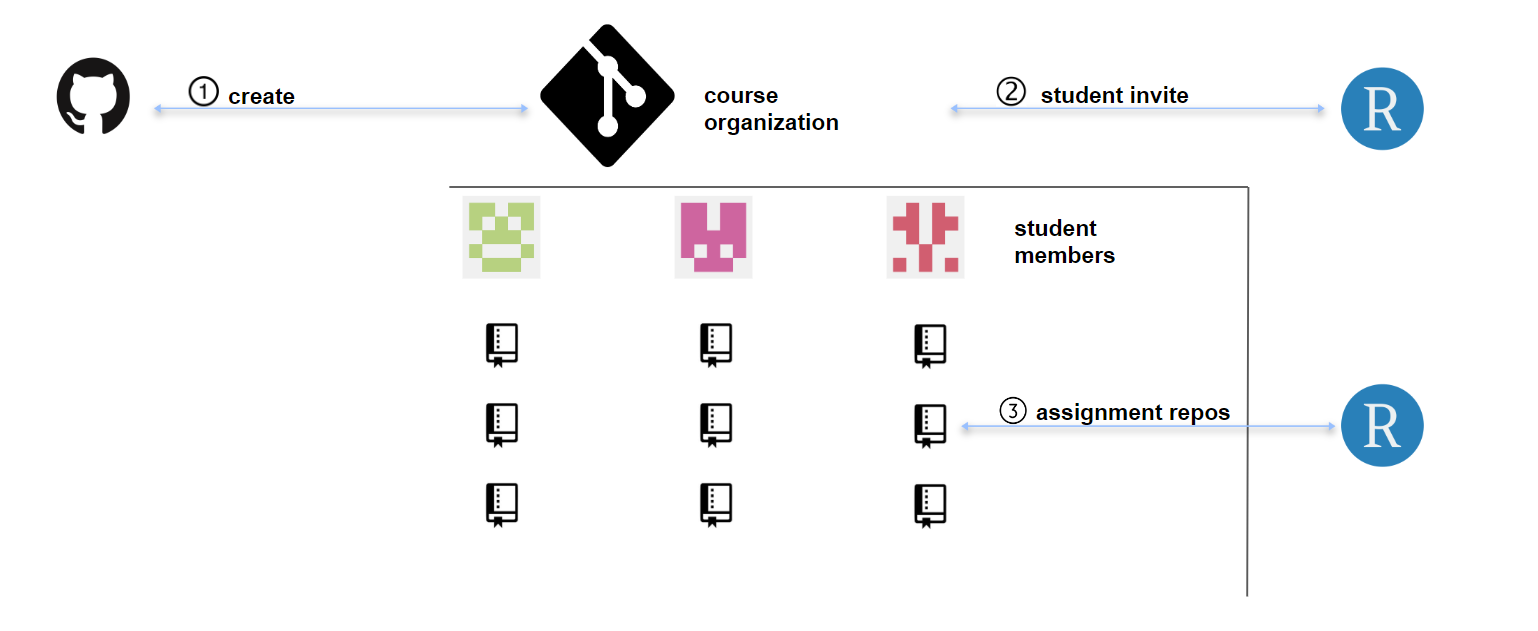
\includegraphics{images/githuborg.png} \textbf{Fig 2:} GitHub
organization structure for STA199

\hypertarget{create}{%
\subsubsection{1. Create}\label{create}}

Using your GitHub account, you can create a new GitHub organization by
clicking on your profile icon in the upper right hand corner, clicking
\emph{Settings}, \emph{Access}, \emph{New Organization}. It's suggested
to name this organization the name of your class and the current
semester you teaching in (i.e., STA 199-s23). Once your organization is
created, you can use packages within R and RStudio to invite students to
enroll.

Supplemental R code to compliment the following sections can be found on
GitHub at (insert GitHub link to code). This includes code on how to
invite students into your personal GitHub organization, and distributing
assessments to students or groups of students via GitHub.

\hypertarget{student-invite-assignment-repositories}{%
\subsubsection{2 \& 3: Student Invite + Assignment
Repositories}\label{student-invite-assignment-repositories}}

STA199 is operated through a GitHub organization where students have the
capability to receive and clone activities onto their personal computer.
To manage and maintain your GitHub organization, we will use a myriad of
functions from the \texttt{gh\_class} package. \textbf{(insert discuss
on what the gh-class package is).}

Students can be invited into your GitHub organization using
\texttt{org\_invite} along with your organization and student GitHub
usernames. Once the invites are sent, students will need to accept the
invitation to the organization. After students have accepted their
invitations, instructors can distribute created assessments to students
within the class GitHub organization by using the function
\texttt{org\_create\_assignment}.

It should be noted that, with such a large class size, \textbf{(time out
error discussion?).}

\textbf{(Code to create ``second batch of AEs'' if needed?)}

Additionally, assessments can be distributed to groups of students
acting as a team (Figure 3).

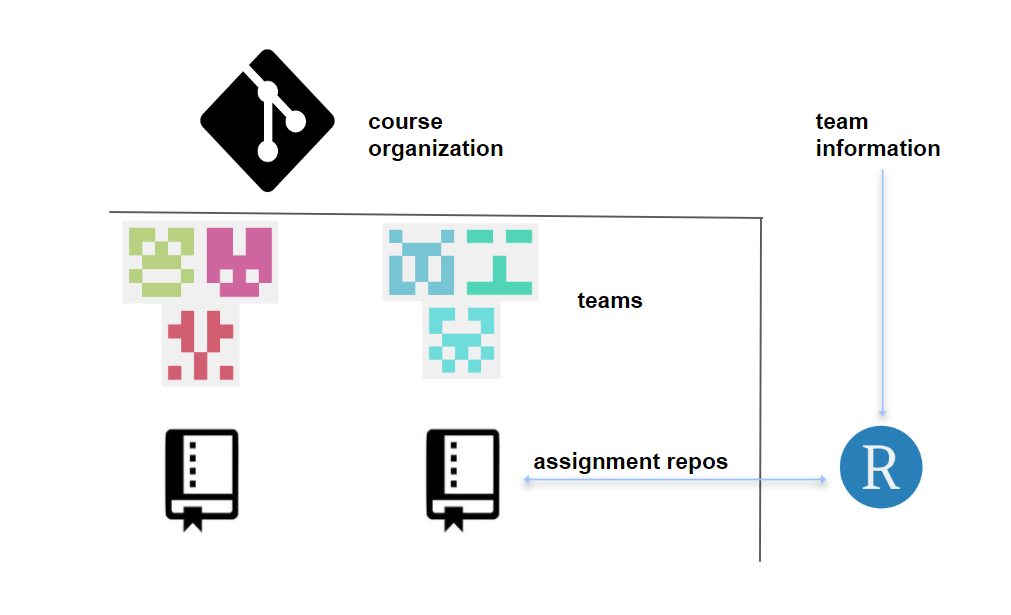
\includegraphics{images/teamorg.png} \textbf{Fig 3:} GitHub organization
structure for team assignments in STA199

This is often advantageous for group projects, and to allow students the
opportunity to use GitHub as a collaboration tool. To accomplish this,
student team information needs to be collected in conjunction with their
GitHub username in a format interpretable using R. We add this
information to the following roster document.

\begin{longtable}[]{@{}llll@{}}
\toprule()
\endhead
team\_name & last\_name & first\_name & github\_username \\
& & & \\
\bottomrule()
\end{longtable}

We can use these new data and change the code found in
\texttt{org\_create\_assignment} function to create repositories for
each team. That is, each individual student will receive a team
repository that each member has access to.

Streamlining your course through R, RStudio, and GitHub greatly
alleviates common challenges that arise when working with a large class
size, such as activity and assessment distribution. How to create an
assignment to distribute is detailed in later sections.

\hypertarget{sec-ped}{%
\section{Pedagogy}\label{sec-ped}}

In the following sections, we discuss pedagogy used within our course,
strategies on how to implement such pedagogy in the classroom, and
detail the creation of assignments such as AEs and lab assessments using
R, RStudio, and GitHub during a typical week in the semester (Figure 4).

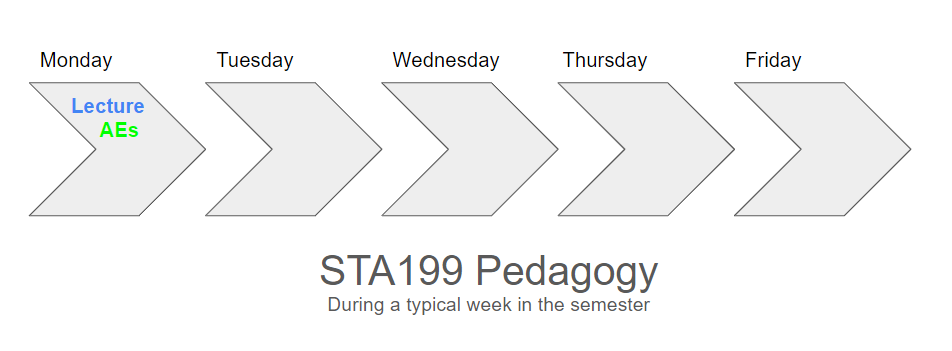
\includegraphics{images/pedagogy.png} \textbf{Fig 4:} Model of
pedagogical choices within the student learning model used in STA 199
for a typical week

In STA 199, we have chosen a combination of teaching methods,
interactive activities, and learning assessments to help prepare
introductory data science students the tools they need to be successful
outside of university or in future coursework. Our pedagogy includes a
combination of lectures, facilitating in-class AEs, and running a lab,
to provide students an opportunity to perform what they've learned.

\hypertarget{lecture-application-exercises}{%
\subsection{Lecture \& Application
Exercises}\label{lecture-application-exercises}}

During a typical week in the semester, class is held twice a week. Class
is a combination of lecture and interactive AEs. The amount of time
dedicated to lecture and AEs can and should vary by instructor.
Typically, we allot the first 15 minutes of class for lecture. During
this time, students are introduced to new content that will be
re-addressed in the AE. To help maximize engagement of such a large
class size, we allot more class time to individual and team-based AEs
where students are asked to code on their own, together, or along with
the instructor. This is followed by a roughly 5-10 minute allotment for
a wrap up lecture, summarizing the highlights of AE.

Application exercises are structured interactive lessons that allow
students to train through doing in class. Students are expected to bring
their laptops to class to participate in AEs. This expectation is made
clear prior to the first day of teaching. The purpose of these exercises
are to give students the opportunity to apply the statistical concepts
and code introduced in the prepare videos, readings, and anything
introduced during lecture.

When first starting to create an AE, we suggest streamlining the process
through a GitHub template repository cloned into RStudio as a project.
We choose to use \emph{Quarto}, within RStudio, to create AEs. This
choice is intentional, to provide students the opportunity to practice
writing code and answering questions in a reproducible format supported
by R and RStudio. When designing questions for an AE, we suggest
creating a mix of coding and concept questions (e.g., fill in the code
blanks, short response questions) that encourage students to follow
along with instructor demonstrations, and also provides students an
opportunity to answer questions on their own. This format has largely
been accepted and appreciated by students: ``I really enjoy the AE's and
that you take the time to walk us through the code and answer questions;
I like how the ae gives us a chance to practice the skills on our own
after class as well.'' Additionally, we suggest that questions are
scaffold, meaning that if students fall behind or type incorrect code
when trying to initially follow along, that they have access to correct
code that grants them the ability to continue engaging for the remaining
AE. This is especially important at the beginning of the semester to
minimize students' frustration around a new coding language. This may
include having answers to questions in a separate Quarto document that
students have access to, or within the same document as the AE.
Moreover, we suggest clearly labeling where students are expected to
type out answers in text or code throughout the exercise to further
streamline their involvement and continue to minimize frustration.

An example of an AE used to help teach \textbf{(insert concept)} can be
found on GitHub here: \textbf{(insert GitHub link)}

We highly recommended designing lessons with built in time to have
students work on their own. The amount of time can largely depend on the
question being asked, and the teaching style of the instructor. We have
found that multiple 3-5 minute blocks for students to answer questions
without the instructor's guidance works well. This has been especially
effective if the code is then created together as a class, built off
student responses, to provide immediate feedback to students before
moving on to the next set of material or questions.

Hands on interactive AEs are the backbone of learning in STA 199. We
have found that providing students with the opportunity to code in
real-time during class keeps them more engaged and eager to continue
learning about the material, versus simply lecturing for a 75-minute
period. This strategy has received positive feedback from students with
varying degrees of coding and statistics experience.

As highlighted in previous sections, this system, streamlined through
GitHub, encourages time investment into the creation of AEs. Investing
time into AE creation provides a strong environment for current students
to learn, and sets a foundation for AEs to be re-tooled instead of
recreated in subsequent semesters. Future renditions of this course can
be modified from previous GitHub organizations efficiently, saving
instructors valuable time and energy before and during the semester.

AEs are designed to be a low stakes assessment where students can earn
full credit by completing in class. Typically, we make AEs worth
completion points that total to be 5\% of a student's end of semester
grade. For students that do not show up to class, we make AEs due three
days from when the AE was assigned. At the end of the semester, if
student's have completed 80\% of AEs, they earn a 100\% for their grade.
Students turn in AEs by pushing their answers within the AE document up
to their GitHub repository. There have been mixed responses from both
students and instructors on assigning a grade to AEs. Disadvantages
include not currently having an efficient way to implement a hard
deadline that students must adhere to, without removing push access from
their AE GitHub repository all-together. Further, if an instructor does
not finish an AE in class, students who did not attend class can be
easily confused on what's expected of them to complete. We suggest
tailoring the decision of grading of AEs to your individual course as
you see fit.

\hypertarget{labs}{%
\subsection{Labs}\label{labs}}

Labs for STA 199 meet once a week for 75 minutes, and are facilitated by
lab leaders and lab helpers. The purpose of labs are to allow students
to apply concepts found in prepare material, lecture, and AEs, to
various data analysis scenarios. Lab section sizes are kept to around 30
students so each have more of an opportunity to converse with each
other, the lab leader, and lab helper, when working through the lab
assessment.

Much like AEs, the instructor or head TA creates and clones a lab GitHub
repository to all students that contains any information and any other
intangibles (like a data set) by changing the \texttt{assignment} object
in the supplemental R code to be the name of original lab GitHub
repository. In a lab GitHub repository, we choose to create a starter
document with places for students to write code under specific question
numbers. The actual lab assessment questions that this repository
corresponds to can be found on the class website that is referenced
during lab time.

Roughly one-third of the way into the semester, students are assigned to
groups to complete a class project. We suggest strategically assigning
groups based on a collection of the following information

\begin{itemize}
\item
  Declared or Intended Major
\item
  Year in School
\item
  Suggested times they work on school assignments
\end{itemize}

From our experience, groups who have significantly different years in
school across students have more friction, and tend to work less well
together than students that have more similar years in school.
Additionally, we highly suggest pairing up students that share common
interests using their intended or declared major in school. The class
project assigned is an open ended research project where the group
collectively decides on a project topic. We have found that students can
feel disengaged or left out of the group if they have different
interests than the others, and their interests are not reflected when
picking a project topic. When groups our assigned, each group during a
lab are tasked to come up with a team name. This team name will be the
name used to create their team repositories for the remaining labs.

From this point forward in the semester, we choose to have all labs be
completed as group work. Introducing group work during labs and through
a class project can help students learn from different perspectives,
practice their communication skills, and improve their problem solving
skills in the context of statistics and data science. The new
expectation is that once groups are formed, one lab assessment will be
turned in for each group instead of each individual. This further helps
lessen the grading responsibilities to those that are assigned it.

After groups are formed, we give a set of recommendations for groups to
help promote a successful and positive group dynamic. This includes:

\begin{itemize}
\item
  Establish a clear line of communication with all members
\item
  Share ideas. Let your voice be heard.
\item
  Teach each other.
\item
  Do not approach group work as a bunch of individual assignments.
\end{itemize}

In our experience, we have observed the use of group work and GitHub
promote teams working in other collaborative platforms to avoid GitHub
merge conflicts. We try to de-incentivise this through multiple avenues.
First, we communicate that each team member must have anywhere from one
to three meaningful commits to the team repository prior to any project
deadline. Secondly, we situate the importance of learning this
collaborative skill in a supportive environment with space to ask
questions and work through such conflicts. Lastly, we demonstrate that
merge conflicts are a part of collaboration using GitHub, and explain
that not all merge conflicts are a ``bad thing.''

To further ensure positive group dynamic, we initiate three peer review
surveys. These peer review surveys provide insight into each group's
dynamic and may inform the teaching team of issues that may need to be
addressed. Questions within each survey range from having only having
instructor only visibility, to being shared with all team members to
promote productive conversations. An example question includes:
\emph{Estimate the percentage of the total amount of work/effort done by
each member, including yourself. Be sure your percentages sum to 100\%!}
We suggest adding additional questions as deemed necessary to help best
understand how everyone is working together within a group.

A new instructor of data science, or one with an increasing class size
should think critically if and how they want to implement group work in
their classroom. In our experience, merge conflicts, the number of
groups, and group formation have been the most difficult aspects of
facilitating group work. Students, especially those newer to coding, are
extremely hesitant to create merge conflicts. Despite a lab dedicated to
the creation and fixing of merge conflicts, students often express
frustration and feel as though they are doing something wrong when merge
conflicts occur. Some groups choose to collaborate using other forms of
technology (e.g., Google documents) before committing and pushing their
finished work onto GitHub. We highly advise against this, and try to
incentivise students by emphasizing the practical importance of learning
how to work through merge conflicts. Secondly, the sheer number of
groups created from 179 students creates an additional time investment
for all members of the teaching team. This includes making sure all
merge conflicts can be fixed accordingly, and helping facilitate an
appropriate working group dynamic among all groups. Finally, there have
been mixed strategies on how to form groups that ultimetely have yielded
similar results. Typically groups are assigned by the instructor using
the aforementioned questions above, while others have allowed students
to select their owns groups. Both strategies have resulted in both
positive and fractured group dynamics. \textbf{(address literature on
group work + group formation?)}. We highly suggest that you consider
additional measures and adjust group formation as you sit fit for your
course.

There are advantages and disadvantages of having lab leaders and helpers
facilitate the lab. Advantages includes having students learning through
additional perspectives, while also providing a potentially more
inviting atmosphere for questions to be asked about the material.
However, disadvantages may include inconsistencies from what is shared
in lab vs lecture. It is critical that lab leaders and helpers are
trained to both understand and explain concepts consistently to what is
being taught during lecture and through the AEs. Additionally we
recommend setting the expectation that lab leaders and helpers become
familiar with the AE content before facilitating the labs so they can
refer students back to resource they are familiar with.

\hypertarget{discussion}{%
\section{Discussion}\label{discussion}}

It is imperative that universities create and implement modernized data
science curricula to both prepare and inspire students to continue their
data science education. This starts with the design and development of
an introductory data science course capable of arming students with the
tools necessary for success in the field. The incorporated technology in
STA 199 able the instructor to efficiently instruct large class sizes
and instill vital skill sets to those who have little to no coding
experience. We believe that this paper helps establish a start to a
consensus while providing a flexible framework for other instructors to
create and facilitate their own introductory data science course. Below,
we unpack critical aspects of the course in an attempt to continue
sharing information that instructors can mold as they see fit.

It is highly advised that live coding sessions be the main staple of
your classroom when teaching students. Live coding sessions continue to
be accepted as one of the best pedagogical practices for teaching coding
\citep{Selvaraj2021}, and have been met in our classrooms with
overwhelming positivity from students: ``\emph{The in-class AEs are
extremely helpful for understanding the concepts and programming};
\emph{aes helped solidify concepts and gave time for practice}; \emph{I
think the ae's are very helpful and I love that it is very hands-on and
easy to follow along}.''

For this to successful, we suggest spending the first couple classes
establishing a routine with your students. This routine ensures that
students clone the live coding exercise (application exercise) prior to
the start of class, and understand that the expectation is to ``learn
through doing'' in live coding sessions.

Despite this suggestion, there are always situations where students can
fall behind in class, limiting the amount of value they may receive from
the exercise. Thus, we have come up with strategies to try and mitigate
the situation. First, the majority of student coding at the beginning of
the semester is done through fill in the blank templates created by the
instructor. This tends to ease tension for those first learning code,
and help instill confidence within students when the code runs.
Secondly, it is suggested to design questions in such a way where there
is little dependency across questions. This means that, if a student
falls behind and is unable to answer one question, this will not deter
them from being involved in upcoming questions. If you do have questions
dependent on each other, we advise providing the answers to the
beginning questions in the same or different document for students to
reference and run so they can continue following along.

With the time investment needed to create enticing and interactive AEs,
it is critical that these resources are easily transferable across
semesters. The design and facilitation of this course is through GitHub.
This ensures that the course content is feasible to adapt to teach for
multiple semesters as classes change and data science continues to
evolve. In short, there is value in the investment to quality resources
early in the classes development, saving time for future renditions.

Additional benefits in deciding to run the course through GitHub help
alleviate the burdens of large class sizes. Using the \texttt{ghclass}
package in R, an instructor can seamlessly distribute homework, labs,
and live coding exercises to as many students as necessary in little
time.

We additionally try and alleviate the challenges of a large class size
with additional computational and human resources. It is not feasible to
expect every student within a large class size to locally install R and
Rstudio for this course. Thus, we suggest using an online platform
capable of hosting R and Rstudio for students. Alleviating initial
frustrations through these means further provide a more inviting
experience to those who have never coded before. If your university does
not provide these measures, we suggest using \emph{RStudio cloud} (do
we?).

Additionally, prompt feedback on assessments is critical in developing
students understanding of R and RStudio. We have decided to implement a
teaching team, and share the responsibility of grading to increase turn
around time. Having a teaching team also provides students multiple
opportunities to receive help on material from a variety of
perspectives. It is understood that having a large teaching team may be
unrealistic, depending on the university resources. In the absence of a
teaching team, it may be advantageous to implement group assignments
even earlier in the semester. This strategy helps mitigate the sheer
quantity of grading from a large class size, as well as lay the
foundation for students to learn coding together from multiple
perspectives.

\newpage

\hypertarget{supplementary-materials}{%
\section{Supplementary materials}\label{supplementary-materials}}

Supplemental materials for the article include\ldots. and can be found
at \ldots{}

\newpage


\renewcommand\refname{References}
  \bibliography{bibliography.bib}


\end{document}
